\documentclass{mcmthesis}


\mcmsetup{CTeX = true,
        tcn = 3700, problem = D,
        sheet = true, titleinsheet = true, keywordsinsheet = true,
        titlepage = false, abstract = true}
\renewcommand{\headset}{{\Large\the\year}\\APMCM\\Summary Sheet}

\usepackage{multirow}
\usepackage{palatino}
\usepackage{lipsum}
\usepackage{indentfirst}
\usepackage{amsmath}
\usepackage{amssymb}
\usepackage{graphicx, subfig}
\usepackage{caption}
\usepackage{booktabs}
\usepackage[section]{placeins}
\usepackage{geometry}
\usepackage{float}
\usepackage{pdfpages}


\geometry{left=1.5cm,right=1.5cm,top=2.5cm,bottom=2.5cm}
\newcommand{\upcite}[1]{\textsuperscript{\textsuperscript{\cite{#1}}}}
%\setlength\parskip{.5\baselineskip}
%\newtheorem{definition}{Definition}[section]

\title{Design of Dater Recommendation Algorithm and Information Forms \\
	with Effect Analysis Study }
%\author{\small \href{http://www.latexstudio.net/}
%  {
\includegraphics[width=7cm]{mcmthesis-logo}}}
%\date{\today}
\begin{document}
\begin{abstract}

\indent
Traditional Internet dating can be quite challening for those singles looking for love. Of all the single men or women met online, very few will be compatible specifically, and it can be difficult to determine the level of compatibility of a potential partner through methods of conventional dating services. This paper adopt K-Means, KNN algorithm and Personality Compatibility Matching Principles to recommend perfect dating partners for people online, devoting to giving a more suitable estimate of an ideally sized choice set and improving success rate of online dating. 

%First of all, we build an AR time series model and use SPSS to build the population growth model in each country on the earth. Then, taking Russian as an example, we divide the countries which use Russian into two parts. One part is called L1 country referred to the country which has Russian as native language. The other is called L2 country referred to the country which has Russian as second language. Next, we remove the two kinds of people including the immigrants and those with low education level in L1 country. For L2 country, we use PCA model to find out the percentage of the people in Russian. Finally we solve the sum and make a prediction that the total speakers of Russian are 162 million. Besides, based on our basic model we also predict the total numbers of speakers of ten languages in 50 years and arrive at the conclusion that the top ten languages will not be replaced.
%
%Secondly, we build a Mechanics-Migration Rate(MMR) model which is inspired by graph theory and mechanics theory. Based on MMR model, we give a immigration transfer matrix of forty countries in every year(���÷���). We take the existing data into the immigration transfer matrix and obtain a figure graph(����ͼƬ)which shows that MMR model is reasonable and feasible. Based on the model above, we find that only a few languages like English will be increased in some regions and we have given some reasonable explanations.
%
%Thirdly, in order to find the optimal location of six offices, we divide the world into eight parts according to some factors and choose ten alternative sites. Then based on the p-median problems, we use LINGO to solve the model. For further study we take two elements into consideration. It is found that the office quantity and scale can be reduced in areas with better development degree. Thus we suggest reducing the number of offices. Last but not least, we conducted a sensitivity test on the established linear programming model.
%
%In short, our model is a reasonable model which can predict the distribution of various languages in the future.
\begin{keywords}
K-Means; K-Nearest Neighbor; Personality Compatibility Matching  \\
\indent\enspace\enspace\enspace\enspace\enspace\enspace\enspace\enspace\enspace\enspace\enspace\enspace Perfect Dating Partner Online Recommendation System
\end{keywords}
    \end{abstract}

 \begin{figure}[!htbp]
	\centering
	%\includegraphics[width = 15cm]{qm.pdf}
	\includepdf{qm.pdf}
	
	\label{qm}
\end{figure}
\newpage
 \begin{figure}[!htbp]
	\centering
	%\includegraphics[width = 15cm]{qm.pdf}
	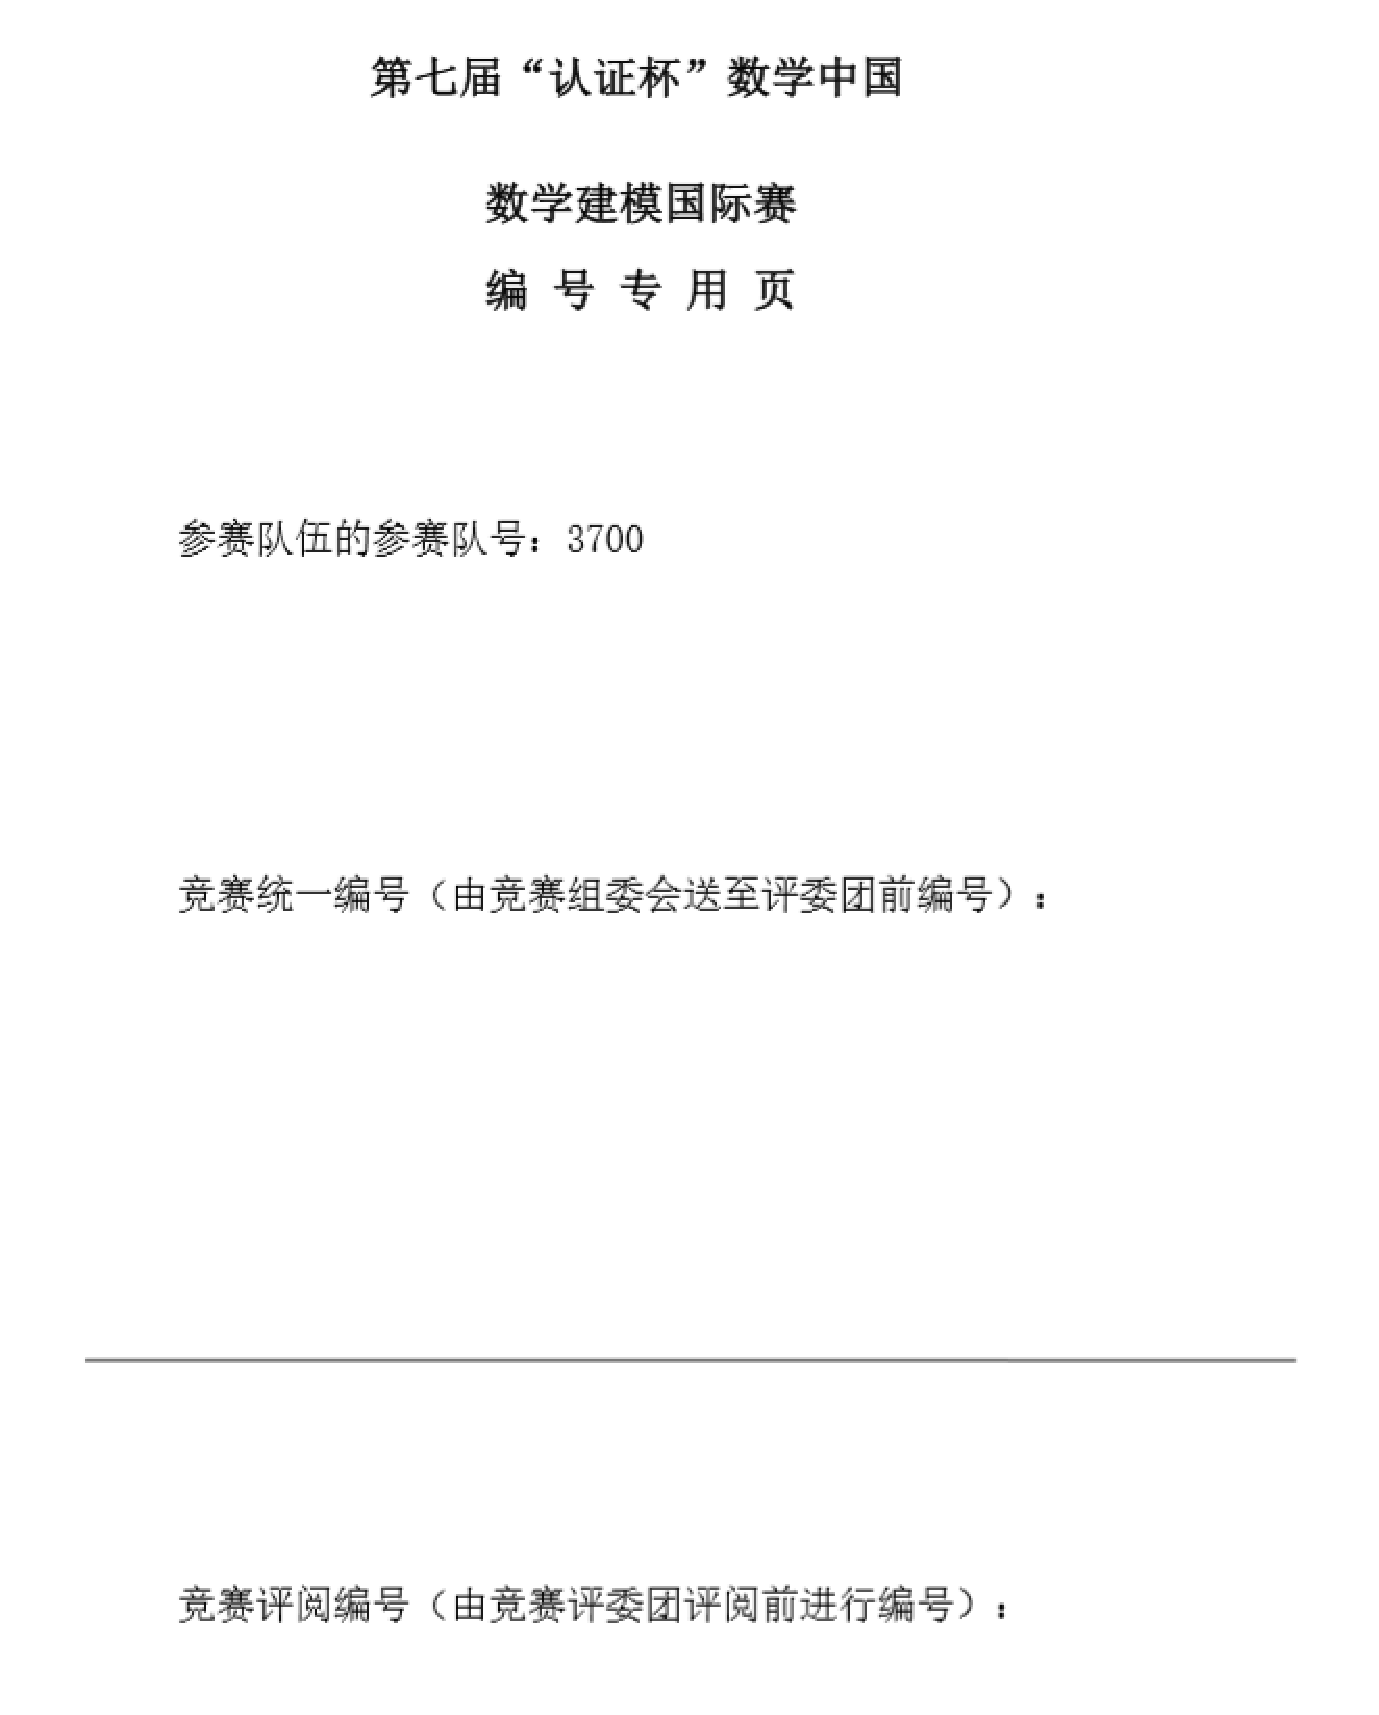
\includepdf{bh.pdf}
	
	\label{qm}
\end{figure}
\newpage

    \maketitle

    \newpage                                %����Ŀ¼
    \setcounter{page}{3}                    %����Ŀ¼
    \tableofcontents                        %����Ŀ¼
    \newpage                                %����Ŀ¼

    \section{Introduction}
    \subsection{Background}                         % ��������
    There are 6,000 to 7,000 languages being used all over the world currently, but around half of the world's population are using the most important 15 languages. With the development of globalization, the whole world has changed deeply. The impact of this trend does not only exist in economy and society, but also in language and culture. Nowadays, with the continuous improvement of transportation and communication, most people are able to speak the second language besides the mother language, and the second language plays an important role in traveling abroad and international trade.
    \begin{figure}[!htbp]                                           %��һ��ͼƬ�ij���
        \centering
        \includegraphics[width = .8\textwidth]{introduction.jpg}        %�ģ�ͼƬ�ļ�������
        \caption{The Distribution of Various Language}                                  %�ģ�ͼƬ����������ʾ������
        \label{introduction}                                           %�ģ�ͼƬ�ڳ����е����ƣ����õ�ʱ����
    \end{figure}

    The current geographical distribution of different languages in the world is shown in the figure \ref{introduction}. When considering the total number of language speakers, native speakers, the second language speakers and even the third language speakers should be taken into consideration. The language distribution is complex and diverse, so the statistics on the total number of languages are a complicated job. At present, many experts and scholars have conducted research in this area to explore whether the trend of language distribution tends to be simplification.
    \subsection{Restatement of the Problem}                  % ǰ�˵Ĺ���
    For the increase of the total number of language speakers, we divided them into native speakers and second language speakers for model building. For the geographical distribution of language speakers, we should not only consider the population increase in each country after 5 years, but also the number of speakers who moving to other countries. Analyzing of the various factors of the problem, we consider the problem how to select the site of the International Office in each country as a risk-based site selection analysis:
This problem can be divided into four parts:
    \begin{itemize}         %û�к����ֵ�
      \item Establish an increase model of the total number of language speakers changed with time to predict the change in the total number of language speakers in the next 50 years.
      \item Establish linguistic geography distribution model changed with time and predict the change of the geographical distribution of the language speakers in the next 50 years.
      \item According to the geographical distribution of language speakers, select the international offices to maximize the profits of the office.
      \item Consider changes in the global communication methods and determine whether the number of international offices can be reduced.
    \end{itemize}


    \subsection{Our Work}                           % ������Ҫ���Ĺ���
    In order to make the prediction more accurate, our work is divided into the following four aspects:
        \begin{figure}[!htbp]                                           %��һ��ͼƬ�ij���
        \centering
        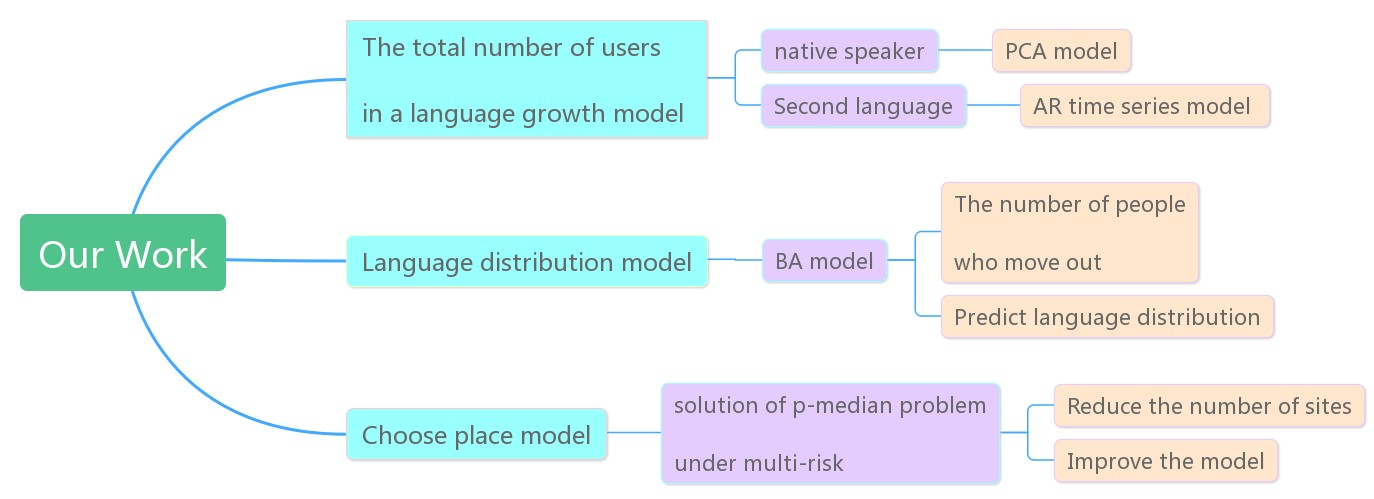
\includegraphics[width = .8\textwidth]{ourwork.jpg}        %�ģ�ͼƬ�ļ�������
        \caption{Flow Chart}                            %�ģ�ͼƬ����������ʾ������
        \label{ourwork}                                           %�ģ�ͼƬ�ڳ����е����ƣ����õ�ʱ����
    \end{figure}


\section{Terminology Explained in Model}        % �൱����������
    \begin{itemize}         %û�к����ֵ�
      \item Nodes centrality degree: The number of edges connected to that node.
      \item L1 country: Countries referred to the country which has Russian as native language.
      \item L2 country: Countries referred to the country which has Russian as second language.
      \item L1 numbers: The numbers of native speakers of a certain language.
      \item L2 numbers: The numbers of second language speakers of a certain language.
    \end{itemize}


\section{Assumptions}
1. We assume that each country uses only the third and fourth languages with very few people, which has little effect on native speakers and second language speakers;

2. We do not consider small probability events in our model, assuming no random events such as world war and economic crisis.

3. Assuming that each country moves in and out of balance, that is, the total population does not change;

4. Assuming that the total number of immigrants to a country speaks the official language of the country and does not consider the issue of the offspring after the move;

5. Assume that all immigrants are legal immigrants;

6. Assuming that national policy does not change significantly over time;

7. Assumptions data are all true and reliable;

\section{Symbols and Definitions}
    \begin{table}[]
    \centering
    \caption{Symbols and Definitions}
    \begin{tabular}{llllll}
             \toprule
        \multicolumn{1}{c}{Symbols} & Meanings                                                                  \\
        \midrule
        ${Y_t}$                     & A country's L1 number                                                         \\
        $\Delta Y(t)$               & the number of population growth one year                                       \\
        $W(t)$                      & A country's L2 speakers                                                       \\
        $S(t)$                      & The population of the country                                                  \\
        ${O_i}$                     & The total degrees of country $i$                                               \\
        ${F_i}(t)$                  & \begin{tabular}[c]{@{}l@{}}The  thrust of\\   country $i$\end{tabular}       \\
        ${N_j}(t)$                  & The attractive force of country $i$                                            \\
        $N{`_i}(t)$                 & \begin{tabular}[c]{@{}l@{}}The tensile force\\   of country $i$\end{tabular}  \\
        ${Q_i}(t)$                  & The total number of people removed from country $i$                            \\
        $R$                         & The total expected value of a local profit                          \\
              \bottomrule
        \end{tabular}
    \end{table}

\section{Simulation Model}                                    % ģ�ͷ�������
    \subsection{Justification of Our Approach}



        \subsubsection{Justification of our approach}
            \begin{itemize}     %��������
                \item \textbf{Why do we build the population growth model?}\\         %ע����ڻ��з��ż���ȥ����
        If we want to model the distribution of language speakers in the future, building the population growth model is necessary because the numbers of different language speakers is changing over time. If we don`t consider this, we can not do the next step and the result must be unreliable.
                \item \textbf{Why do we divide each language into different country?}\\  % ע����ڻ��з��ż���ȥ����
        Because different country has different population growth rule and different L2 country has different proportion of L2 speaker. If we easily add up the native language and the second language and make a simple calculation of population growth model, the error of result is very big.
                \item \textbf{Why do we divide each language into two parts(L1 country, L2 country)?}\\
        It is obviously that L1 country and L2 country have different rule about calculating the proportion of the speakers of a particular language. So what we need do is to find the population of every country which speaks a particular language, and find the proportion of this language in these countries.
            \end{itemize}




    \subsubsection{Basic Model}
    1) AR Time Series Model

In order to get a model which have the ability to predict, we build an AR Time Series Model. Autoregressive model is:
\[\Delta {{\rm{Y}}_{\rm{t}}}{\rm{ = }}{\alpha _{\rm{0}}}{\rm{ + }}\sum\limits_{{\rm{i = 1}}}^n {{\alpha _i}\Delta {Y_{i - 1}} + {\mu _i}} \]


where ${{\alpha }_{0}}$. is constant, ${{\alpha }_{i}}$ is coefficient of the model, ${{\mu }_{i}}$ is White Noise Sequence.

As an analogy, the model of population growth is:

\begin{equation}\label{renkouzengzhang}
  {Y_t} = {Y_{t - 1}} + \Delta {Y_t}
\end{equation}
where ${{Y}_{t}}$ is the population this year, $\Delta {{Y}_{t-1}}$ is the number of population growth, $\left\{ \Delta {{Y}_{t}} \right\}$is first-order difference sequence of the population.

Based on this, the numbers of speakers of a particular language in L1 country are:
\[Y = (1 - \beta  - \lambda ){Y_t}\]
Where $\beta $ is the proportion of immigrant this year,$\lambda $ is the proportion of people with a low level of literacy. $n$is the number of L1 country.

2) PCA Model



    \[\left\{ \begin{array}{l}
{F_1} = {a_{11}}{X_1} + {a_{12}}{X_2} + {a_{13}}{X_3} + {a_{14}}{X_4}\\
{F_2} = {a_{21}}{X_1} + {a_{22}}{X_2} + {a_{23}}{X_3} + {a_{24}}{X_4}\\
{F_3} = {a_{31}}{X_1} + {a_{32}}{X_2} + {a_{33}}{X_3} + {a_{34}}{X_4}\\
{F_4} = {a_{41}}{X_1} + {a_{42}}{X_2} + {a_{43}}{X_3} + {a_{44}}{X_4}\\
{F_5} = {a_{51}}{X_1} + {a_{52}}{X_2} + {a_{53}}{X_3} + {a_{54}}{X_4}
\end{array} \right.\]




    3) Total Numbers of Speakers
    Total numbers of language speakers of a certain language is:
    \[S(t) = Y(t) + W(t)\]
        \subsubsection{ Solution and Result }
        In this problem we have to model the distribution of various language speakers over time. But due to the wide distribution of languages, we focus on the analysis of the four representative languages which are English, Russian, Chinese, Japanese. We use our model to predict their distribution ten years later.


Figure.\ref{sub1} shows the autocorrelation and partial autocorrelation coefficients of Russia`s population growth function, and Figure.\ref{sub2} shows the population trend ten years after the prediction of Russia.

    \begin{figure}[!htbp]                                       
        \centering
        \subfloat[ACF and PACF]{                               
            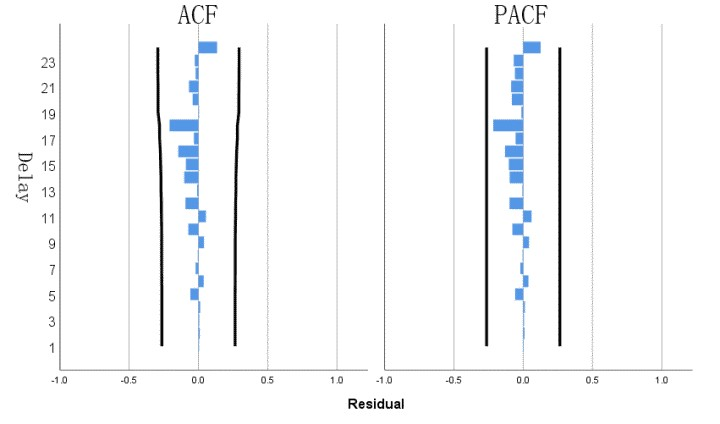
\includegraphics[width = .45\textwidth]{ACF.jpg}
            \label{sub1}                                          
        }
        \qquad
        \subfloat[Change in Russia`s Population]{                            
            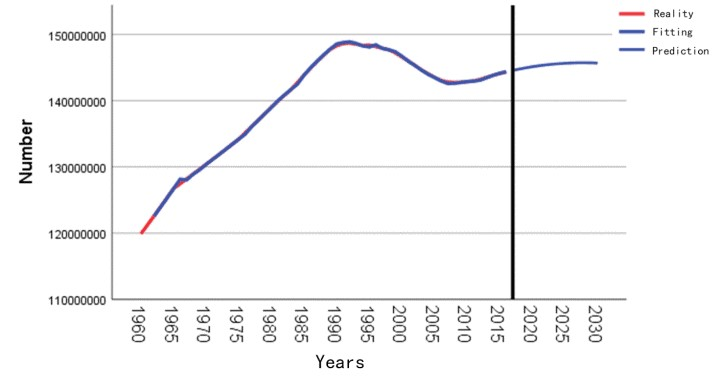
\includegraphics[width = .45\textwidth]{eluosi.jpg}
            \label{sub2}                                            
        }\\ 

        \caption{The Growth Model of Russia`s population}                                       
        \label{eluosibijiaotu}                                 
    \end{figure}

As can be seen from Figure.\ref{eluosibijiaotu}, Russia's total population is 145 million after 10 years. As for $\beta $, $\lambda $ parameter in Equation.\ref{renkouzengzhang}, we find the data from 1960 to 2016 in World bank.

We choose four languages and make a prediction about their L1 speakers number. Result is shown in Table.\ref{Atu}
\begin{table}[H]
\centering
\caption{The Change of L1 Speakers in Four Countries}
\label{Atu}
\begin{tabular}{llllll}
\cline{1-3}
\multicolumn{1}{c}{}        & \multicolumn{1}{c}{Now} & \multicolumn{1}{c}{In ten years} &  &  &  \\ \cline{1-3}
\multicolumn{1}{c}{Russian} & \multicolumn{1}{c}{153} & \multicolumn{1}{c}{162}             &  &  &  \\
\multicolumn{1}{c}{English} & \multicolumn{1}{c}{371} & \multicolumn{1}{c}{405}             &  &  &  \\
\multicolumn{1}{c}{Chinese} & \multicolumn{1}{c}{897} & \multicolumn{1}{c}{955}             &  &  &  \\
\multicolumn{1}{c}{Jpanese} & \multicolumn{1}{c}{128} & \multicolumn{1}{c}{124}             &  &  &  \\ \cline{1-3}

\end{tabular}
\end{table}

As for the number of L2 speakers, we almost find all the certain language`s L2 country and use our model to calculate the number of their L2 speakers in 2017, as is shown in Figure.\ref{AtuL2}. Comparing the result with the actual data in 2017, we find it that our model can basically figure out the number of L2 speakers.
    \begin{figure}[H]                                           %��һ��ͼƬ�ij���
        \centering
        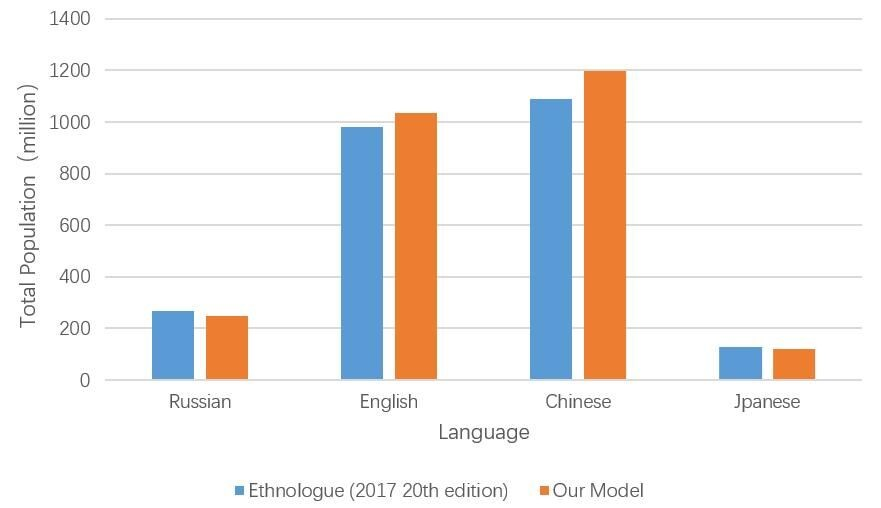
\includegraphics[width = .8\textwidth]{AtuL2.jpg}        %�ģ�ͼƬ�ļ�������
        \caption{Model Test}                            %�ģ�ͼƬ����������ʾ������
        \label{AtuL2}                                           %�ģ�ͼƬ�ڳ����е����ƣ����õ�ʱ����
    \end{figure}

Finally, we predict the total languages speakers of the four languages we choose.

\begin{table}[H]
\centering
\caption{The Total Numbers of Four Languages}
\label{Bjieguo}
\begin{tabular}{cccclcl}
            \toprule
                     & Native Language      &                      & \multicolumn{2}{c}{Second Language}                     & \multicolumn{2}{c}{Total}                               \\
                     \midrule
                     & Now                  & In Ten Years         & Now                  & \multicolumn{1}{c}{In Ten Years} & Now                  & \multicolumn{1}{c}{In Ten Years} \\
Russian              & 153                  & 162                  & 113                  & \multicolumn{1}{c}{119}          & 266                  & \multicolumn{1}{c}{281}          \\
English              & 371                  & 405                  & 611                  & \multicolumn{1}{c}{666}          & 982                  & \multicolumn{1}{c}{1071}         \\
Chinese              & 897                  & 955                  & 193                  & \multicolumn{1}{c}{205}          & 1090                 & \multicolumn{1}{c}{1160}         \\
Jpanese              & 128                  & 124                  & 1                    & \multicolumn{1}{c}{1.2}          & 129                  & \multicolumn{1}{c}{125.2} \\
\bottomrule
\end{tabular}
\end{table}

It can be seen from Table.\ref{Bjieguo} that the total languages speaker change a little after 10 years.

        \subsubsection{Result and Analysis}


\begin{table}[H]
\centering
\caption{The Predictions of 6th-16th Language`s Total Numbers of Speakers}
\label{Bdaan}
\begin{tabular}{ccccccc}
        \toprule
           & \multicolumn{2}{c}{L1} & \multicolumn{2}{c}{L2} & \multicolumn{2}{c}{Total} \\
           \midrule
           & Now    & In 50 Years   & Now    & In 50 Years   & Now     & In 50 Years     \\
Malay      & 77     & 107           & 204    & 271           & 281     & 378             \\
Bengali    & 242    & 340           & 19     & 22            & 261     & 362             \\
Russian    & 153    & 183           & 113    & 158           & 267     & 341             \\
Portuguese & 218    & 297           & 11     & 16            & 229     & 313             \\
French     & 76     & 101           & 153    & 203           & 229     & 304             \\
Hausa      & 85     & 132           & 65     & 93            & 150     & 225             \\
Punjabi    & 148    & 192           &        &               & 148     & 192             \\
German     & 76     & 106           & 52     & 69            & 129     & 175             \\
Persian    & 60     & 84            & 61     & 85            & 121     & 169             \\
Japanese   & 128    & 164           & 1      & 1.3           & 129     & 165.3           \\
Swahili    & 16     & 22            & 91     & 131           & 107     & 153\\
\bottomrule
\end{tabular}
\end{table}


  1. The country corresponding to the top-ten language can be divided into two parts. Some countries have a small population but have developed economically. Some countries have an underdeveloped  economy but have a lager population base.
      \begin{itemize}
        \item As for the first kind of countries like America, they have strong comprehensive national strength so their native language has become world official language, the other country should learn their language to carry out business and other activities.
        \item As for the second kind of countries like China, their people have superiority, so the number of native language is hard to be exceeded by other countries.
      \end{itemize}

  2. Since the countries ranked after the tenth in the rankings are not economy powerhouse and have not a large population base, growth in both native speakers and second language speakers is not high.

      3. We have ignored the small probability events, such as national split, war, invasion by other countries and other factors, so population model is the ideal model, so there will be such a result.



\section{Model II}

    \subsection{Prediction Model}
    1) BA Model



    \begin{figure}[H]                                           %��һ��ͼƬ�ij���
        \centering
        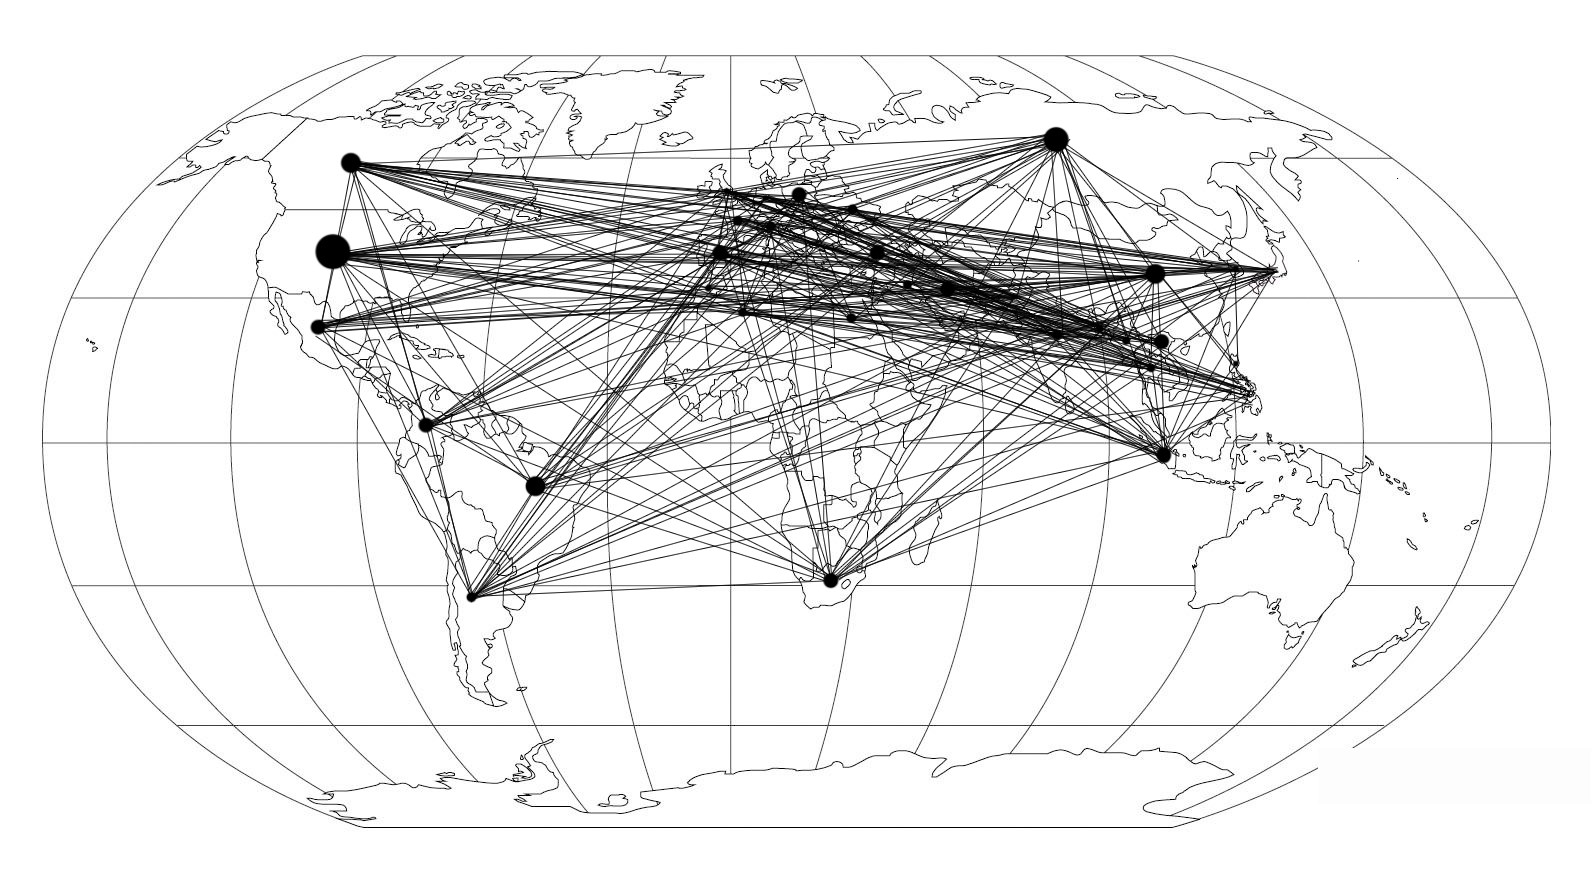
\includegraphics[width = .8\textwidth]{yiduixian.jpg}        %�ģ�ͼƬ�ļ�������
        \caption{Global Population Mobility Network Space Pattern}                            %�ģ�ͼƬ����������ʾ������
        \label{yiduixian}                                           %�ģ�ͼƬ�ڳ����е����ƣ����õ�ʱ����
    \end{figure}





    \subsection{Applications of Our Models}

\section{Strengths and Weaknesses}
    \subsection{Strengths}
        \begin{itemize}
            \item
            \item
            \item
        \end{itemize}
    \subsection{Weaknesses}
        \begin{itemize}
            \item
            \item
            \item
        \end{itemize}

\begin{thebibliography}{99}                 % ���Dz����
    \bibitem{1}
    \bibitem{2}
    \bibitem{3}
    \bibitem{4}
\end{thebibliography}

\begin{appendices}
	
	\section{First appendix}

	
	Here are simulation programs we used in our model as follow.\\
	
	\textbf{\textcolor[rgb]{0.98,0.00,0.00}{Input matlab source:}}
	\lstinputlisting[language=Matlab]{./code/mcmthesis-matlab1.m}
	
	\textbf{\textcolor[rgb]{0.98,0.00,0.00}{Input python source:}}
	\lstinputlisting[language=Python]{./code/feature.py}
	
	\section{Second appendix}
	
	some more text \textcolor[rgb]{0.98,0.00,0.00}{\textbf{Input C++ source:}}
	\lstinputlisting[language=C++]{./code/mcmthesis-sudoku.cpp}
	
\end{appendices}
\end{document}

                        %��������
\end{document}
